\documentclass[12pt, a4paper]{article}

\usepackage[a4paper, top=2cm, bottom=3cm, left=2cm, right=2cm]{geometry}
\usepackage[export]{adjustbox}
\usepackage{graphicx}
\usepackage{mathtools}
\usepackage{hyperref}
\usepackage{amsmath}
\usepackage{amsfonts}
\usepackage{amssymb}
\usepackage[version=4]{mhchem}
\usepackage{stmaryrd}
\usepackage{polyglossia}
\usepackage{fontspec}
\usepackage{ucharclasses}
\usepackage{fancyhdr}
\usepackage{wrapfig}
\usepackage{subcaption}
\usepackage{relsize}
\usepackage{framed}
\usepackage{changepage}
\usepackage{tabularray}
\usepackage{etoolbox}
\usepackage{xstring}
\usepackage{pstricks-add}
\usepackage{tikz}
\usepackage{empheq}
\usepackage{tcolorbox}
\usepackage[european,s traightvoltages, americanresistor, americaninductors]{circuitikz}
\usepackage{pgfplots}
\usepackage{tikz-3dplot}

\usetikzlibrary{
	angles,
	arrows.meta,
	positioning,
	arrows,
	backgrounds,
	calc,
	decorations,
	decorations.markings,
	decorations.pathmorphing,
	fit,
	shapes.arrows,
	shapes.callouts,
	shapes.geometric,
	shapes.misc,
	snakes,
	quotes
}
\pgfplotsset{compat=1.18}
\hypersetup{colorlinks=true, linkcolor=blue, filecolor=magenta, urlcolor=cyan,}
\urlstyle{same}

\setmainlanguage{english}
\setotherlanguages{norwegian, arabic}
\newfontfamily\arabicfont{Noto Naskh Arabic}
% \newfontfamily\lgcfont{CMU Serif}

%%%%%%%%%% Fancy header %%%%%%%%%
\pagestyle{fancy}
\fancyhead[C]{}
\fancyfoot[C]{\medskip\thepage}
\renewcommand{\footrulewidth}{.4pt}
\renewcommand{\headrulewidth}{0pt}

\setlength{\headheight}{14.49998pt}
\addtolength{\topmargin}{-2.49998pt}

\newcommand{\figwidth}{8cm}
\newcommand{\floatfigwidth}{5cm}


%%%%%%%%%% Formatters & Layout %%%%%%%%%
\newcommand{\uprimary}[1]{
	\section*{\center \Huge \underline{#1}}
	\addcontentsline{toc}{section}{\protect\numberline{}#1}
}
\newcommand{\usecondary}[1]{
	\section*{\center \LARGE \underline{#1}}
	\addcontentsline{toc}{section}{\protect\numberline{}#1}
}
\newcommand{\usection}[1]{
	\section*{\LARGE #1}
	\addcontentsline{toc}{subsection}{\protect\numberline{}#1}
}
\newcommand{\usubsection}[1]{
	\section*{\Large #1}
	\addcontentsline{toc}{subsection}{\protect\numberline{}#1}
}
\newcommand{\ussubsection}[1]{
	\section*{\large #1}
	\addcontentsline{toc}{subsection}{\protect\numberline{}#1}
}
\newcommand{\ans}{\bigskip\underline{\textbf{Answer}}}
\newcommand{\ques}[1]{\noparindent\textbf{#1}\doparindent}
\newcommand{\rfloatingimg}[1]{
	\begin{wrapfigure}{r}{\floatfigwidth}
		\includegraphics[max width=\floatfigwidth]{#1}
	\end{wrapfigure}
}
\newcommand{\indentbox}[2]{
	\begin{adjustwidth}{#1}{0pt}
		#2
	\end{adjustwidth}
}
\newcommand{\qa}[3]{
	\noparindent
	\textbf{#1 #2}
	\indentbox{.76cm}{
		\ans
		#3
	}
	\vspace{.75cm}
}
\newcommand{\noskipqa}[2]{
	\noparindent
	\textbf{#1}
	\indentbox{.76cm}{
		\ans
		#2
	}
}
\newcommand{\eqnleft}[1]{
	\begin{flalign*}
		 & #1 &  &
	\end{flalign*}
}
\newcommand{\fullwidthimg}[1]{
	\begin{center}
		\includegraphics[max width=\textwidth]{#1}
	\end{center}
}
\newcommand{\uheading}[2]{
	\uprimary{Module - #1}
	\vspace{-.7cm}
	\usecondary{#2}
}

\newcommand{\note}[1]{
	\begin{tcolorbox}[colframe=green!40!black, colback=green!5!white, title={\textbf{Note}}]
	#1
	\end{tcolorbox}
}


%%%%%%%%%% general constants/symbols %%%%%%%%%
\newcommand\longUparrow{\mathrel{\scalebox{1}[2]{$\uparrow$}}}
\DeclareRobustCommand{\rchi}{{\mathpalette\irchi\relax}}
\newcommand{\irchi}[2]{\raisebox{\depth}{$#1\chi$}}
\newcommand{\term}[1]{\underline{\textbf{#1}}}
\newcommand{\amstr}{\mathring{\textrm{A}}}
\newcommand{\h}{6.626 \times 10^{-34}}
\newcommand{\kB}{1.38 \times 10^{-23}}
\newcommand{\lc}{3 \times 10^{8}}
\newcommand{\uunit}[1]{\mathrm{~#1}}

%%%%%%%%%% Format constants %%%%%%%%%
\newcommand{\doparindent}{\setlength\parindent{.5cm}}
\newcommand{\noparindent}{\setlength\parindent{0pt}}
\graphicspath{ {../images/} }
\NewDocumentCommand{\multiskip}{m}{%
	\begingroup
	\newcount\i  % Define a new counter \i
	\i=0         % Initialize the counter
	\loop
	\ifnum\i<#1
	\bigskip  % Add \bigskip
	\advance\i by 1  % Increment the counter
	\repeat
	\endgroup
}

\newcommand{\termlist}[1]{
	\begin{tcolorbox}[colback=blue!10!white, colframe=blue!50!black, title={Some terms}]
		#1
	\end{tcolorbox}
}


%%%%% dev fx
% startx, starty, endx, endy
\newcommand{\dottedgrid}[4]{
	\draw[thin, dotted] (#1, #2) grid (#3,#4);
	\foreach \i in {#1,...,#3} \node at (\i,-2ex) {\i};
	\foreach \i in {#2,...,#4} \node at (-2ex,\i) {\i};
}
\newcommand{\smallmidarrow}[2]{\tikz \draw[arrows = {-Straight Barb[scale=.8]}, line width=#1] (0,0) -- +(#2,0);}
\newcommand{\midarrow}[2]{\tikz \draw[arrows = {-Straight Barb[scale=1.1]}, line width=#1] (0,0) -- +(#2,0);}

\DefTblrTemplate{caption-tag}{default}{}
\DefTblrTemplate{caption-sep}{default}{}
\DefTblrTemplate{caption-text}{default}{}
\DefTblrTemplate{contfoot-text}{default}{}
\DefTblrTemplate{conthead-text}{default}{}
\begin{document}
\uheading{1}{Lasers \& Fibre optics}
\usection{Laser}
$\sim$ Light amplification by stimulated emission of radiation
- (others: Maser, Eraser).

\usubsection{Characteristics}
\begin{enumerate}
	\item \term{Monuchromaticity}\\
	      Has extremely narrow bandwidth. $\Delta \lambda=5 \times 10^{-14} \unit{m}$ (conventional light source: 1000 $\amstr$)\\
	      Degree of monochromaticly: $\varepsilon=\frac{\Delta\lambda}{\lambda}$ \ \ ($\Delta\lambda \Rightarrow$ spead of light)
	\item \term{Directionality}\\
	      Can travel large distances with minimal deviation.\\
	      Divergence $\Delta \theta=\frac{r_2-r_1}{D_2-D}$ or $D^2 / \lambda$ (Reliegh's range) \\
	      For laser: $10 \mu\unit{rad}$\\
	      for search light $0.5rad$
	      $>\Rightarrow$ divergence
	\item \term{Coherence}\\
	      \textbf{Spatial coherence}:when a when wave maintains constant phase difference at two points on the wave over a time ($t$).

	      \textbf{Temporal coherence}: when there is no phase change at a point on the wave over a time. (these reference points are taken on electric field)
	\item \term{Brightness/intensity}\\
	      Laser produce highly intense beams, because more light energy is concentrated in a small region. Also laser light is coherent, so at a time many photons are in phase. They superimpose to produce a wave of larger amplitude. Hence resultant intensity  $\propto$amplitude$^2$) is very high.
\end{enumerate}

\noparindent
\begin{framed}
	\indentbox{0.75cm}{
	\term{Coherence length ($L_c$)}:Propagation distance over which a coherent wave maintains a specified degree of coherence or phase difference \\
	for He-Ne: 600km


	\term{Coherence time($\tau_c$)}: time over which a propagating wave remains coherent or the maximum time interval for which the wave have definite phase relation. \\
	For He-Ne: $\tau_c=2 \times 10^{-3} \unit{s}$\\
	Sodium lamp: $10^{-10} \unit{s}$\\
	\term{non-chromaticity $\propto L_c^{-1}$}
	}
\end{framed}


\usubsection{Spontaneous \& stimulated emission}
\fullwidthimg{laser-1}

\ussubsection{Spontaneous emission}
Atom initially at excited state makes transition voluntarily on its own, without aid of any external agency, to ground state, and emits photon of energy $$h \nu_{12}=E_2-E_1$$
Different atoms of medium emits light at different times and different directions. Hence emitted photons are incoherent.

\ussubsection{Stimulated emission}
Here photon having energy $h\nu_{12}(=E_2-E_1)$ impinges on (or passes in the vicinity of) an atom present in its excited state and atom is stimulated to make transition to ground state and gives off a photon of energy $h \nu_{12}$. Emitted photon in is in phase with the incident photon. These two travel in same direction and posses same frequency. They're coherent.

\usubsection{Einstein's coefficients}
For a system containing atoms and radiation, ratio of atoms in ground state($N_1$) to atoms in excited state($N_2$) is:
$$
	\frac{N_2}{n_1}=e^{-\frac{E_2-E_1}{k_B T}} = e^{-\frac{h \nu}{k_B T}}
$$
\begin{itemize}
	\item When atom in ground state gets excited to higher state, rate or absorption of radiation is : $B_{12} n_1 \rho_{v_{12}}$ ($\rho_{v_{12}}=$ energy density of incident radiation)
	\item Rate of spontaneas emission: $R_{21}=N_2 A_{21}$
	\item Rate of absorption : $R_{12}=N_1 \rho_{v_{12}} B_{12}$
	\item Rate of stimulated emission: $R_{21}=N_2 \rho_{v_{12}} B_{21}$
\end{itemize}
Where

$N_1=$ number of availoble atoms per unit volume

$B_{12}=$ probability of absorpion per unit time

$A_{21}=$ probability that atom will spontaneously jump to $E_1$ (ground state). per unit time.

$N_2 =$ number of atoms per unit volume
$B_{21}=$ probability that atom will transition from $E_2$ to $E_1$ via stimulated emission per unit time

\begin{framed}

	\lefteqn{\rho_v=\frac{8 \pi h \nu^3}{c^3} \times \frac{1}{e^{h\nu/(kT)}-1}}

	Consider a 2 level energy system $E_1 \& E_2$ with only spontaneous emission.

	At thermal equibrium, rate of absorption = rate of emission.
	\bigskip

	\lefteqn{\rho_{v_{12}} B_{12} N_1=A_{21} N_2 \Rightarrow \rho_{V_{11}}=\frac{A_{21} N_2}{B_{12} N_1}=\frac{A_{21}}{B_{12}} e^{-\frac{E_2 - E_1}{kT}}}

	\bigskip

	But it's not in accordance with $\rho_v$.

	For this, Einstein proposed Stimulated emission:

	At Thermal Equilibrium. rate of absorption = rate of emission:

	\lefteqn{B_{12} \rho_{v_{12}} N_1 = A_{21} N_2 + B_{21} \rho_{v_{21}} N_2}

	% \begin{flalign*}
	% 	\Rightarrow \rho_{V_{12}} & =\frac{A_{21} N_2}{B_{12} N_1 - B_{21} N_2}                                                                                                                              &  & \\
	% 	                          & =\frac{A_{11}}{B_{12} e^{h\nu/(kT)} - B_{21}}                                                                                                                                 \\
	% 	                          & =\frac{A_{21}}{B_{21}} \cdot \frac{1}{\frac{B_{12}}{B_{21}} \left(e^{h\nu/(kT)} - 1\right)}                                                                              &  & \\
	% 	                          & \Rightarrow B_{12} \approx B_{21}, \quad \frac{A_{21}}{B_{21}}=\frac{S_p \cdot E_m}{51 \cdot G_m}=8 \pi                                                                  &&   \\
	% \end{flalign*}
	\begin{flalign*}
		\frac{A_{21}}{B_{21}}  =\frac{\text{probability of spontaneas emission}}{\text{probability of stimulated emission}} & =\frac{8 \pi h \nu^3}{c^3}           &  & \\
		                                                                                                                    & =\frac{8 \pi h c^3 / \lambda^3}{c^3} &  & \\
		                                                                                                                    & =\frac{8 \pi h}{\lambda^3}           &  &
	\end{flalign*}
	\begin{flalign*}
		\frac{R_{21}}{R_{21}} & =\frac{\text{Rate of spontaneas emission}}{\text{Rate of stimulated emission}} =e^{h\nu/(kT)}-1 &
	\end{flalign*}

\end{framed}

\ussubsection{\small{Note:}}
\begin{itemize}
	\item Spontaneous emission produce incoherent light
	\item Stimulated emission produce coherent light
\end{itemize}

\usubsection{Population Inversion}
\begin{itemize}
	\item When photon of Energy $\Delta E$ (equal to difference in energy level) enters atom\\
	      probability of absorption = probability of spontaneas emission
	\item At Room temperature: $\Delta E = E_2-E_1 \approxeq 0.025 \unit{eV}$ (Corresponding to IR radiation of $6 \times 10^{12} \unit{Hz}$)
\end{itemize}

\term{Population inversion}: Is is a state of system in which more members of system are in high energy level than in lower level.
\fullwidthimg{pi}

At thermal equibrium: $N\left(E_2\right) / N\left(E_1\right)=e ^ {-\left(E_2-E_1\right) / (kT)}$

\term{pumping}: Supplying energy to excite atoms to upper levels.

\usubsection{Purity of spectral line}

Finite purity or sharpress $=\frac{\lambda}{\Delta \lambda}$

$\Delta \nu / \Delta\lambda=$ Spread of frequency.

Fading of amplitude is explained by setting $\Delta\nu$ in time $\tau_c$ by unity:
$$
	\begin{aligned}
		 & \tau_c \Delta \nu=1 \Rightarrow \Delta \lambda=\frac{\lambda^2}{\tau_c c} \\
		 & L=c \tau_c=\frac{\lambda^2}{\Delta \lambda}= \lambda Q
	\end{aligned}
$$

For Sodium line: $\Delta \lambda = 0.12\amstr$
For He-Ne laser $\Delta \lambda = 0.0005 0.12\amstr$

\bigskip

\qa{1}{For a source of monochromatic radiation with wavelength 5000$\amstr$, and frequency $6 \times 10^{14} \unit{Hz}$, what will be the sharpress for conventional light with $\Delta \nu=10^{10} \unit{Hz}$ and les with $\Delta \nu=500\unit{Hz}$ ?}
{
For conventional radiation:
\lefteqn{\frac{\Delta \nu}{\nu}=\frac{10^{10}}{6 \times 10^{14}}=1.67 \times 10^{-5}}

For laser:
\lefteqn{\frac{\Delta \nu}{\nu}=\frac{500}{6 \times 10^{14}}=6 \times 10^{-12}}
}

\qa{2}{For a He-Ne laser, Output diameters are 4 nm and 5 nm at distances 1m and 2m. Calculate beam divergence}
{
	Beam divergence
	\lefteqn{=\frac{R_2-R_1}{D_2-D_1}=\frac{.5\unit{mm}}{1 \unit{m}}=\frac{1}{2} 10^{-3} \unit{rad}}
}

\qa{3}{For ordinary source of light, $\tau_c=10^{-10} \unit{s}$. Obtain its sharpness if wavelength is 5400$\amstr$}
{
\begin{flalign*}
	Q                              & =\frac{\Delta \nu}{\nu}
	\nu                            & =\frac{c}{\lambda}=5.56 \times 10^{14} \unit{Hz}                         &  & \\
	\tau_c                         & =\frac{1}{\Delta\nu} \Rightarrow \Delta \nu=1 / \tau_c=10^{10} \unit{Hz} &  & \\
	\therefore \text { Sharpness } & =\frac{10^{10}}{5.56 \times 10^{14}}=1.8 \times 10^{-5}
\end{flalign*}
}

\qa{4}{A monochromatic source emits light of wavelength 5461$\amstr$. Its bandwidth $\Delta \nu=10^9$Hz. Find $\tau_c, L_c$ and frequency stability (sharpness)}
{
	\begin{flalign*}
		 & \tau_c=\frac{1}{\Delta v}=10^{-9} s                                                              &  & \\
		 & L_c=\tau_c c=30 \unit{cm}                                                                        &  & \\
		 & \nu=\frac{c}{\lambda}=5.49 \times 10^{44} \unit{Hz}                                              &  & \\
		 & \text { Sharpress }=\frac{\Delta \tau}{\nu}=\frac{10^9}{5.49 \times 10^{14}}=1.82 \times 10^{-6} &  &
	\end{flalign*}
}

\usubsection{Representing transitions}
\begin{itemize}
	\item Absorption: $A+h\nu \rightarrow A^{*}$
	\item Spontaneous Emission: $A^{*} \rightarrow A+h\nu$
	\item Stimulated Emission : $A^{*}+h\nu \rightarrow A+2 h\nu$
\end{itemize}
$\star$ Emitted photon is identical to incident one. (have same frea, phase, polarisation)

$\star$ Since excited states are highly unstable (atom will returns to ground state in less than 1ns) an intermedioute energy level (which has life time of $10^{-3}$ to $10^{-4}$s) is required to create stimulated emission. This is achieved by using certain dopants.

\usubsection{Fabrication of laser}
\begin{center}
	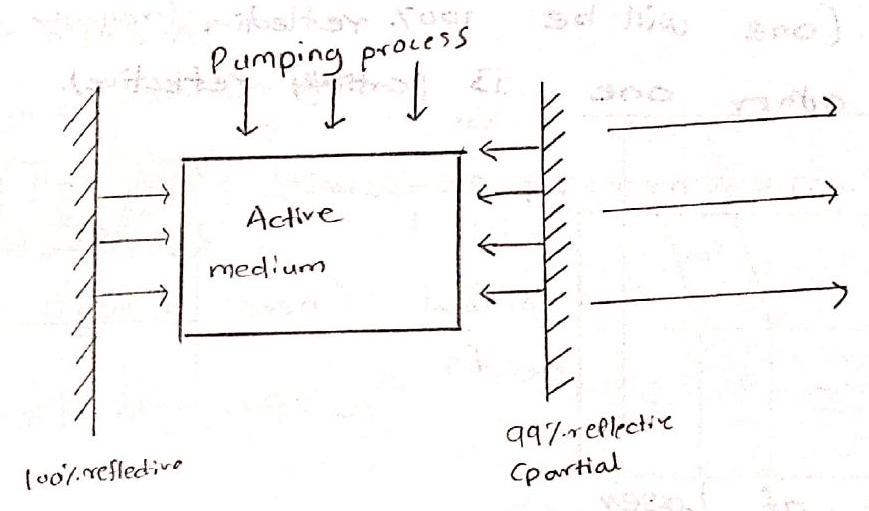
\includegraphics[max width=\textwidth]{2024_06_16_30d750483617f1939202g-02}
\end{center}

\term{Active medium}: material in which popalation inversion takes place. (eg. ruby)

\term{Active center}: Atoms which can produce more stimulated emission than spontaneous emission: (e.g: Cr in ruby, Ne in He-Ne medium).

\term{Pumping mechanism}: Adding energy to system. This can be done by:
\begin{itemize}
	\item Optical pumping (used in ruby laser, xe-flash lamp)
	\item Direct electron excitation.
	\item Inelastic atom-atom collisions: electric discharge is employed to cause collision and excitation of atoms. (used in He-Ne)
	\item Chemical reactions.

\end{itemize}

\usubsection{Optical resonance \& Resonance cavity}

Two mirrors are used to reflect light back into active medium one will be 100 \% reflective.(Usually made of dielectic material) and other one is partially reflective.

Two arrangements of mirrors are used to reflect light:
\begin{itemize}
	\item \textbf{plane-parallel}: needs to be strictly parallel (with deviation less than 1" (1/3600$^{\deg}$)) and must have smooth surface(irregularities <1/100$\lambda$).
	\item \textbf{confocal}: need to be parallel (with deviation less than 0.025$^{\deg}$)
\end{itemize}


\ussubsection{Types of Laser}

\begin{itemize}
	\item \textbf{Pulsed mode}: Train of pulses are produced. It can have produce power in the order of 1MW.
	\item \textbf{Continuous mode}: Light is produced continuously. It has less powerful output (less than 1W) (eg: He-Ne laser)
\end{itemize}


\usubsection{Ruby Laser}

\begin{itemize}
	\item Created in 1960 by maiman
	\item It is a 3 level system
	\item Produced light in pulsating maner (continuous mode not possible due to heating of active medium)
	\item Active medium: $\mathrm{Al}_{2} \mathrm{O}_{3} \cdot \mathrm{Cr}^{3+}$ (0.05-0.5 \% of Al atoms are replaced with Cr atoms)
	\item Eavelength of light emitted: 6943 $\amstr$
\end{itemize}

\begin{center}
	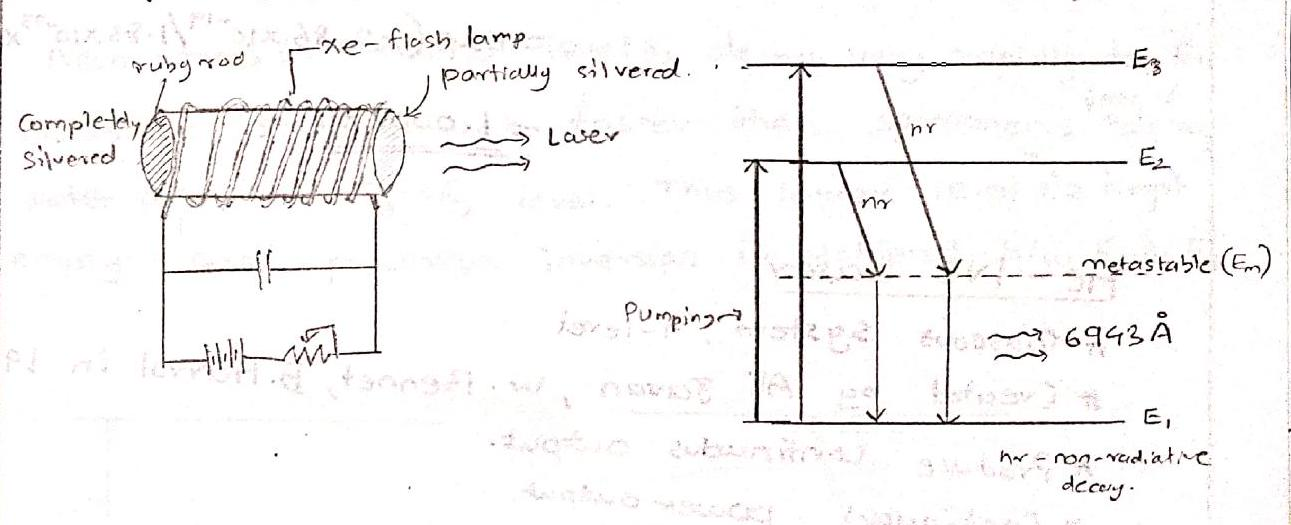
\includegraphics[max width=\textwidth]{2024_06_16_30d750483617f1939202g-03(1)}
\end{center}

$\star$ Population inversion is achieved b/w E$_m$ \& E,
\pagebreak
\begin{figure*}
	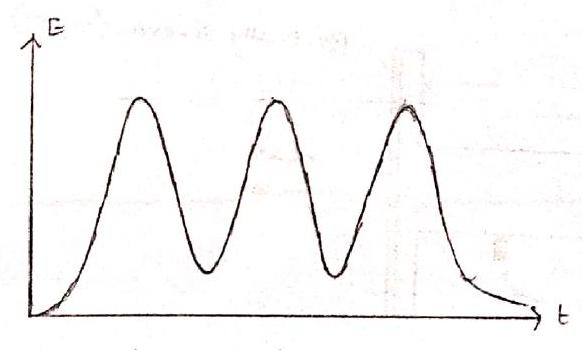
\includegraphics[max width=.5\linewidth]{2024_06_16_30d750483617f1939202g-03}
	\caption*{Intensity us time graph}
\end{figure*}

\ussubsection{Working of Ruby laser}
Cr$^{3+}$ ions absorb pumping light and go to excited states E$_2$ \& E$_3$. From these a rapid radiationless transition to the metastable level E$_m$ takes place. Decay from E$_m$ is very slow that with sufficient excitation, populations inversion between E$_m$ \& E$_1$ can occur. Those photons are allowed to pass millions of times in the active medium with the help of mirrors. When threshold conditions are. satisfied, an intense pulse of light of wavelength 6934$\amstr$ is emitted. Continuous operation is not possible due to excessive heating of active medium.

\bigskip

\qa{1}{For semiconductor, band gap is 0.9eV, what is wavelength of light emitted from it?}
{
	\begin{flalign*}
		h\nu               & = 0.9 \unit{eV} = 1.442 \times 10^{-19}\unit{~J}                     &  & \\
		\therefore \nu     & = \frac{1.442 \times 10^{-19}}{h}                                    &  & \\
		                   & = \frac{1.442 \times 10^{-19}}{\h} = 2.176 \times 10^{14} \unit{~Hz} &  & \\
		\therefore \lambda & = c / \nu         = 1.38\unit{~\mu m}                                &  & \\
	\end{flalign*}
}
\qa{2}{For a He-Ne laser with wavelength 632.8 nm and output power 3.14 mW how many photons are emittal in each minute in operation?}
{
	\begin{flalign*}
		\text{Energy of each photon } = h\nu & = \frac{hc}{\lambda}                       &  & \\
		                                     & = \frac{\h \times \lc}{632.8\time 10^{-9}} &  & \\
		                                     & = 3.14 \times 10^{-19} \unit{~J}           &  &
	\end{flalign*}
	\begin{flalign*}
		\therefore \text { Energy emitted in 1 minute } & = 3.14 \unit{~mW} \times 60 = 0.1884\unit{J}        &  & \\
		\therefore \text { Number of photons emitted }  & =\frac{0.1884}{3.14 \times 10^{-19}}=6\times10^{17} &  & \\
	\end{flalign*}
}

\end{document}
